\documentclass[tikz,border=2pt]{standalone}
\usepackage{amsmath,amssymb}
\usepackage{tikz}
\usetikzlibrary{arrows.meta}

\begin{document}
% The same vector w has different coordinates in different bases: (3.8, 2) in the standard
% basis, (2, 1) in the basis (b1, b2) = ((1.4, 0.5), (1, 1)).
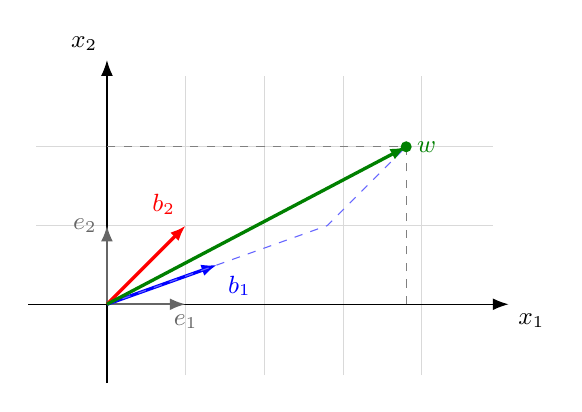
\begin{tikzpicture}[every node/.style={font=\small}, >={Latex[length=2mm]}]
	\draw[gray!30, step=1] (-0.9,-0.9) grid (4.9,2.9);
	\draw[->] (-1,0) -- (5.1,0) node[below right] {$x_1$};
	\draw[->] (0,-1) -- (0,3.1) node[above left] {$x_2$};
	\draw[->, gray!80!black, thick] (0,0) -- (1,0) node[below] {$e_1$};
	\draw[->, gray!80!black, thick] (0,0) -- (0,1) node[left] {$e_2$};
	\draw[->, blue, very thick] (0,0) -- (1.4,0.5) node[below right] {$b_1$};
	\draw[->, red, very thick] (0,0) -- (1,1) node[above left] {$b_2$};
	\draw[dashed, blue!60] (0,0) -- (2.8,1.0) -- (3.8,2.0);
	\draw[dashed, gray] (3.8,0) -- (3.8,2.0) -- (0,2.0);
	\draw[->, green!50!black, very thick] (0,0) -- (3.8,2.0) node[right] {$w$};
	\fill[green!50!black] (3.8,2.0) circle (2pt);
\end{tikzpicture}
\end{document}
